\section{Results}

\subsection{Summary of Data and Model Selection}

Environmental factors, but not wind, drove monarch abundance changes in 1,894 paired observations from 115 monitoring periods at two overwintering sites during the 2023-2024 season. Testing of 47 candidate models identified M23 as the best-fit model.

Model M23 included smooth terms for previous butterfly count, temperature, butterflies in direct sun, and time since sunrise, achieving an AIC value of 8081.848 (Table~\ref{tab:model_selection}). This model accounted for 88\% of the model weight (AIC weight = 0.88), with the next-best model (M22) showing substantially less support (ΔAIC = 4.796). Notably, model M24, which included maximum wind speed as an additional predictor, performed worse than M23 (ΔAIC = 6.2), and wind variables appeared in none of the top-performing models.

\begin{table}[htbp]
\centering
\caption{Model selection results showing the top five candidate models ranked by AIC. Model terms are shown with their respective AIC values, ΔAIC relative to the best model, and AIC weights. Wind p-values are shown where applicable; NA indicates the model did not include wind variables.}
\label{tab:model_selection}
\begin{tabular}{lllrrr}
\hline
Model & Terms & AIC & ΔAIC & Weight & Wind p \\
\hline
M23 & Previous butterfly count, Temperature, & 8081.8 & 0.0 & 0.880 & NA \\
    & Butterflies in direct sun, Time since sunrise & & & & \\
M22 & Previous butterfly count, Temperature (linear), & 8086.6 & 4.8 & 0.080 & NA \\
    & Butterflies in direct sun, Time since sunrise & & & & \\
M24 & Previous butterfly count, Maximum wind speed, & 8088.0 & 6.2 & 0.040 & 0.218 \\
    & Temperature, Butterflies in direct sun, Time since sunrise & & & & \\
M47 & Temperature, Butterflies in direct sun, & 8101.3 & 19.4 & <0.001 & NA \\
    & Time since sunrise & & & & \\
M17 & Previous butterfly count, Temperature, & 8105.9 & 24.0 & <0.001 & NA \\
    & Butterflies in direct sun & & & & \\
\hline
\end{tabular}
\end{table}

\subsection{Analysis of the Best-Fit Model}

The best-fit model (M23) explained 5.7\% of variance in monarch abundance changes (adjusted R² = 0.057). The model formula was:

\begin{equation}
\text{Change in abundance} \sim s(\text{Previous butterfly count}) + s(\text{Temperature}) + s(\text{Butterflies in direct sun}) + s(\text{Time since sunrise})
\end{equation}

where $s()$ denotes smooth terms. All four smooth terms showed significant effects on monarch abundance changes.

\begin{table}[htbp]
\centering
\caption{Summary of smooth terms in the best-fit model (M23). EDF represents effective degrees of freedom, indicating the complexity of each smooth relationship.}\label{tab:smooth_terms}
\begin{tabular}{lrrrr}
\hline
Term & EDF & Ref.~df & F-value & p-value \\
\hline
Previous butterfly count & 2.62 & 2.62 & 12.02 & 8.26e-07 \\
Temperature & 3.93 & 3.93 & 3.23 & 0.028 \\
Butterflies in direct sun & 1.53 & 1.53 & 19.36 & 1.22e-05 \\
Time since sunrise & 4.90 & 4.90 & 8.90 & <2e-16 \\
\hline
\end{tabular}
\end{table}

The previous butterfly count showed a significant non-linear negative relationship with abundance change (EDF = 2.62, F = 12.02, p < 0.001). As the previous count increased, the change in abundance became increasingly negative, indicating proportionally greater departures from larger aggregations (Figure~\ref{fig:effect_roost_size}). Temperature exhibited a complex non-linear relationship (EDF = 3.93, F = 3.23, p = 0.028), with effects peaking at approximately 20°C (Figure~\ref{fig:effect_temperature}).

\begin{figure}[htbp]
\centering
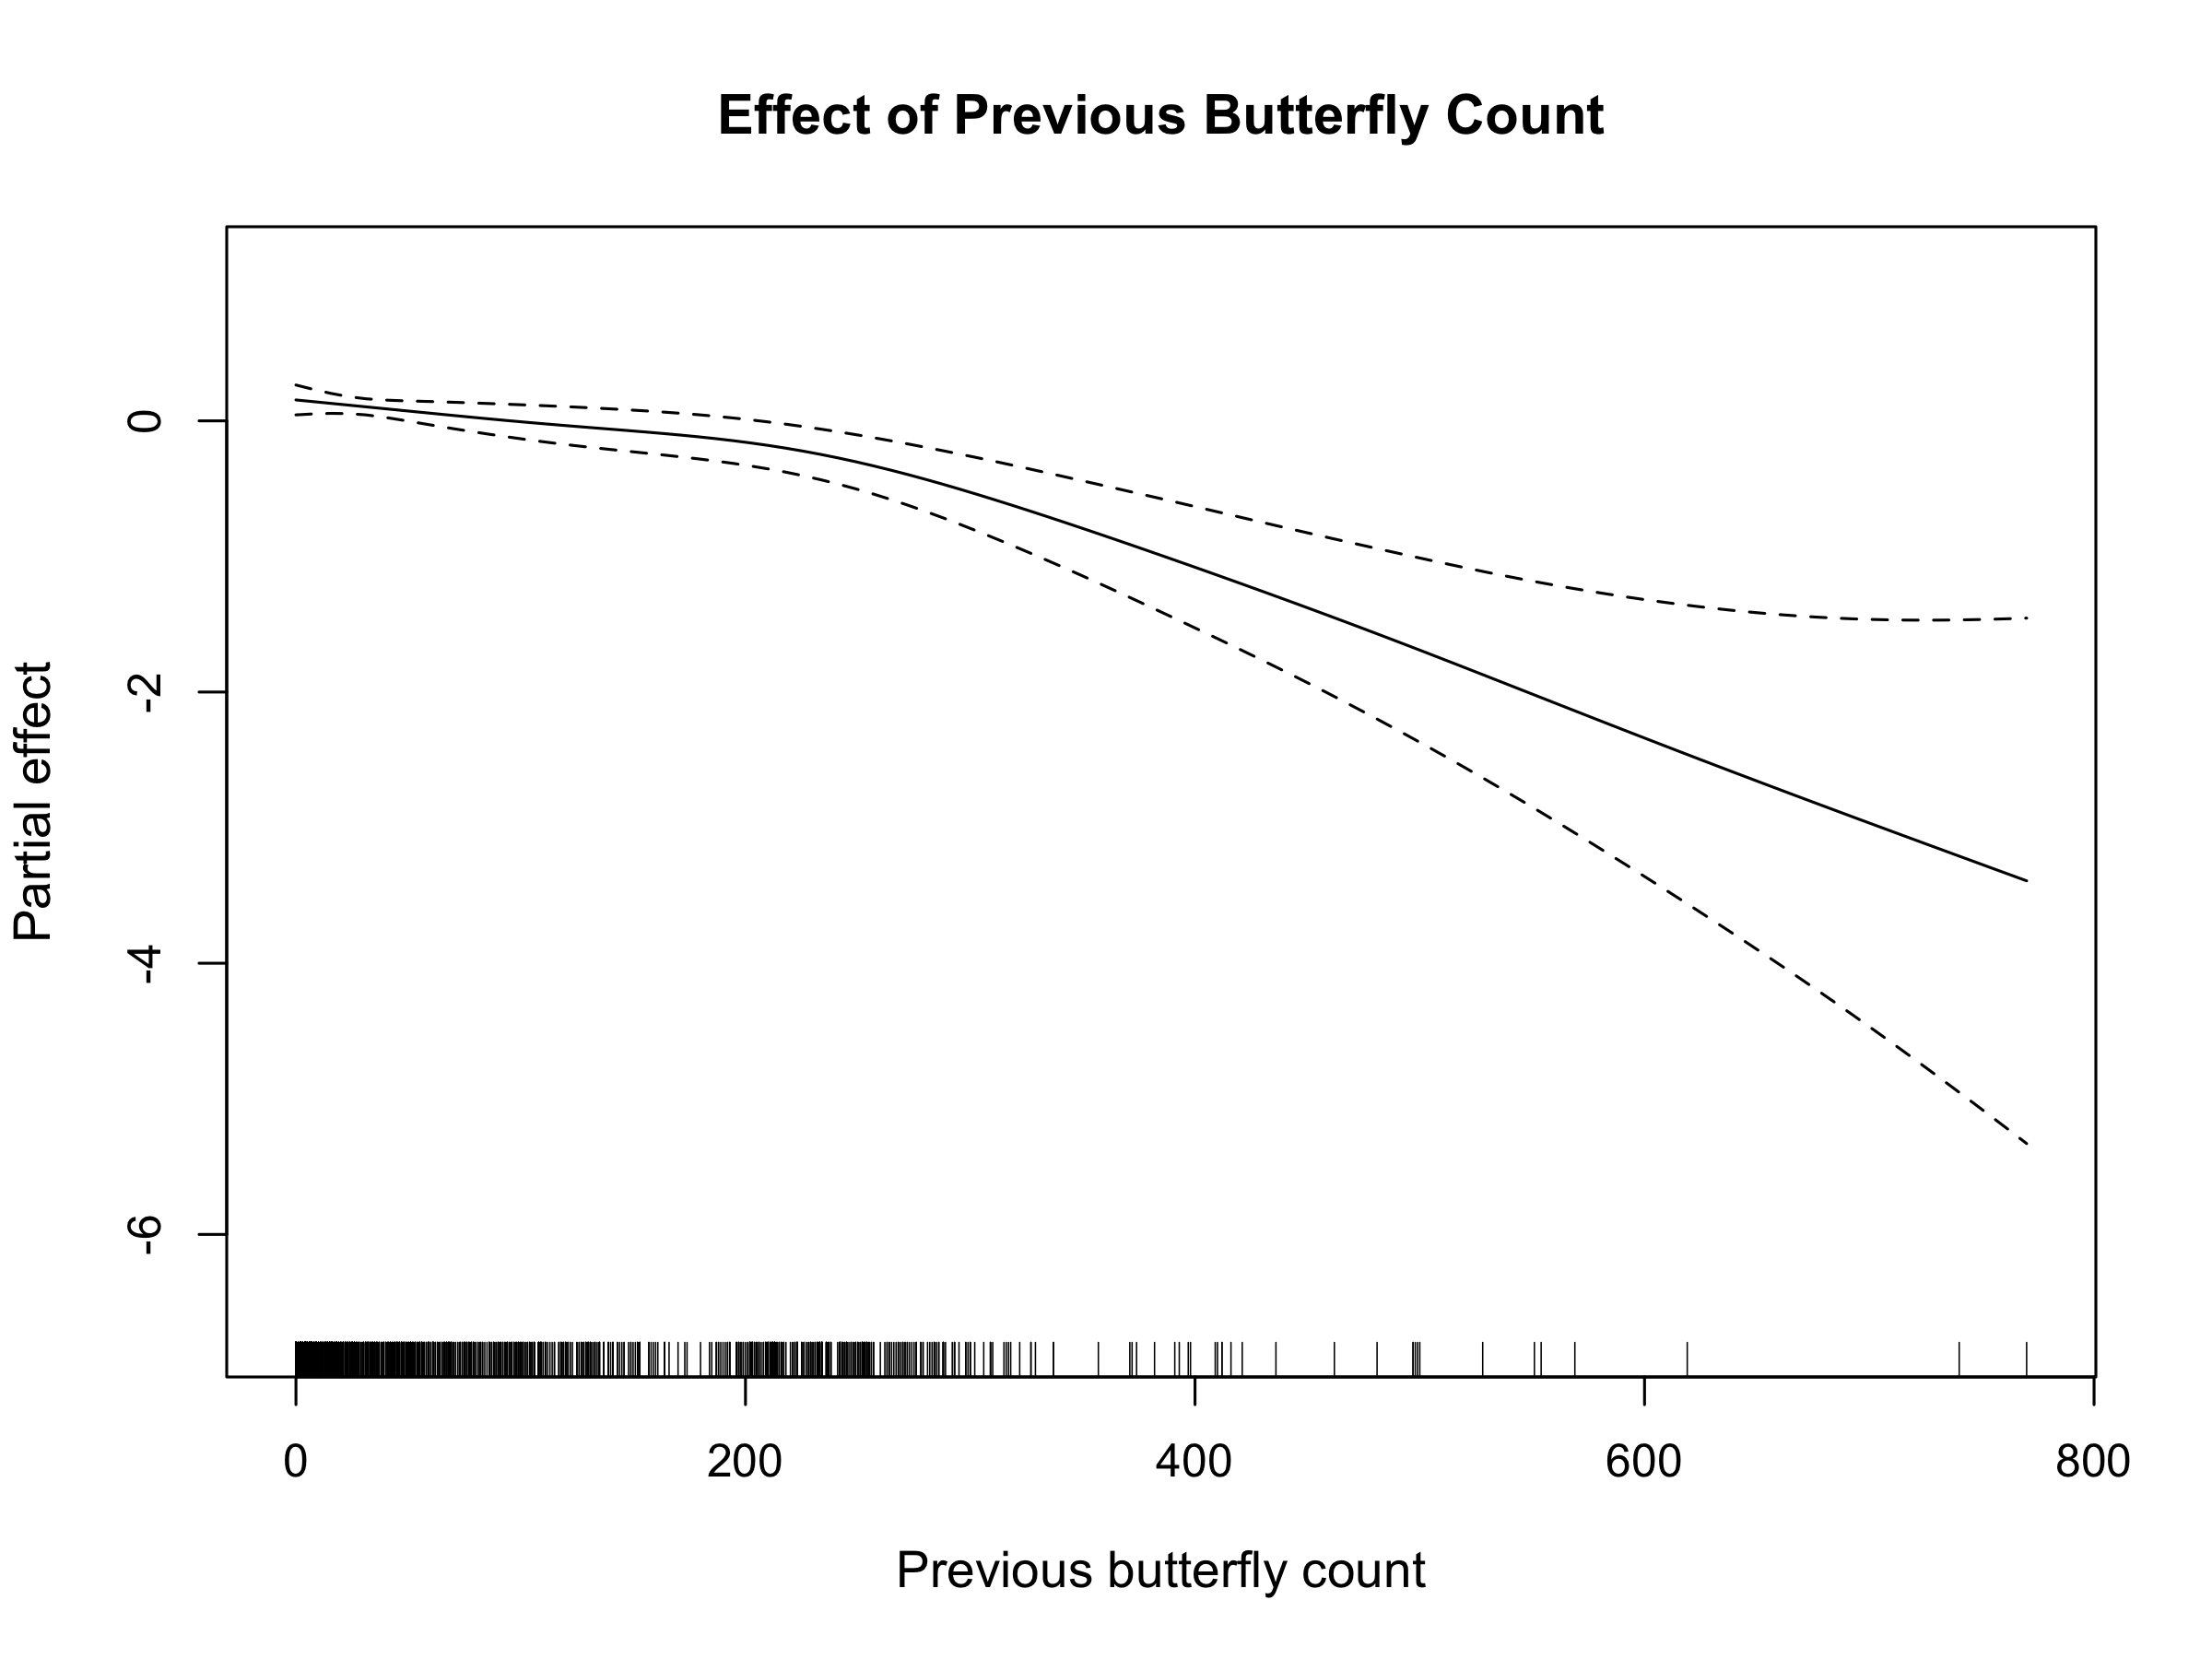
\includegraphics[width=0.8\textwidth]{supplemental/results/thesis_exports/figures/effect_previous_butterfly_count.png}
\caption{Partial effect of previous butterfly count on abundance change, showing greater departures from larger roosts. Shaded area: 95\% confidence interval.}\label{fig:effect_roost_size}
\end{figure}

\begin{figure}[htbp]
\centering
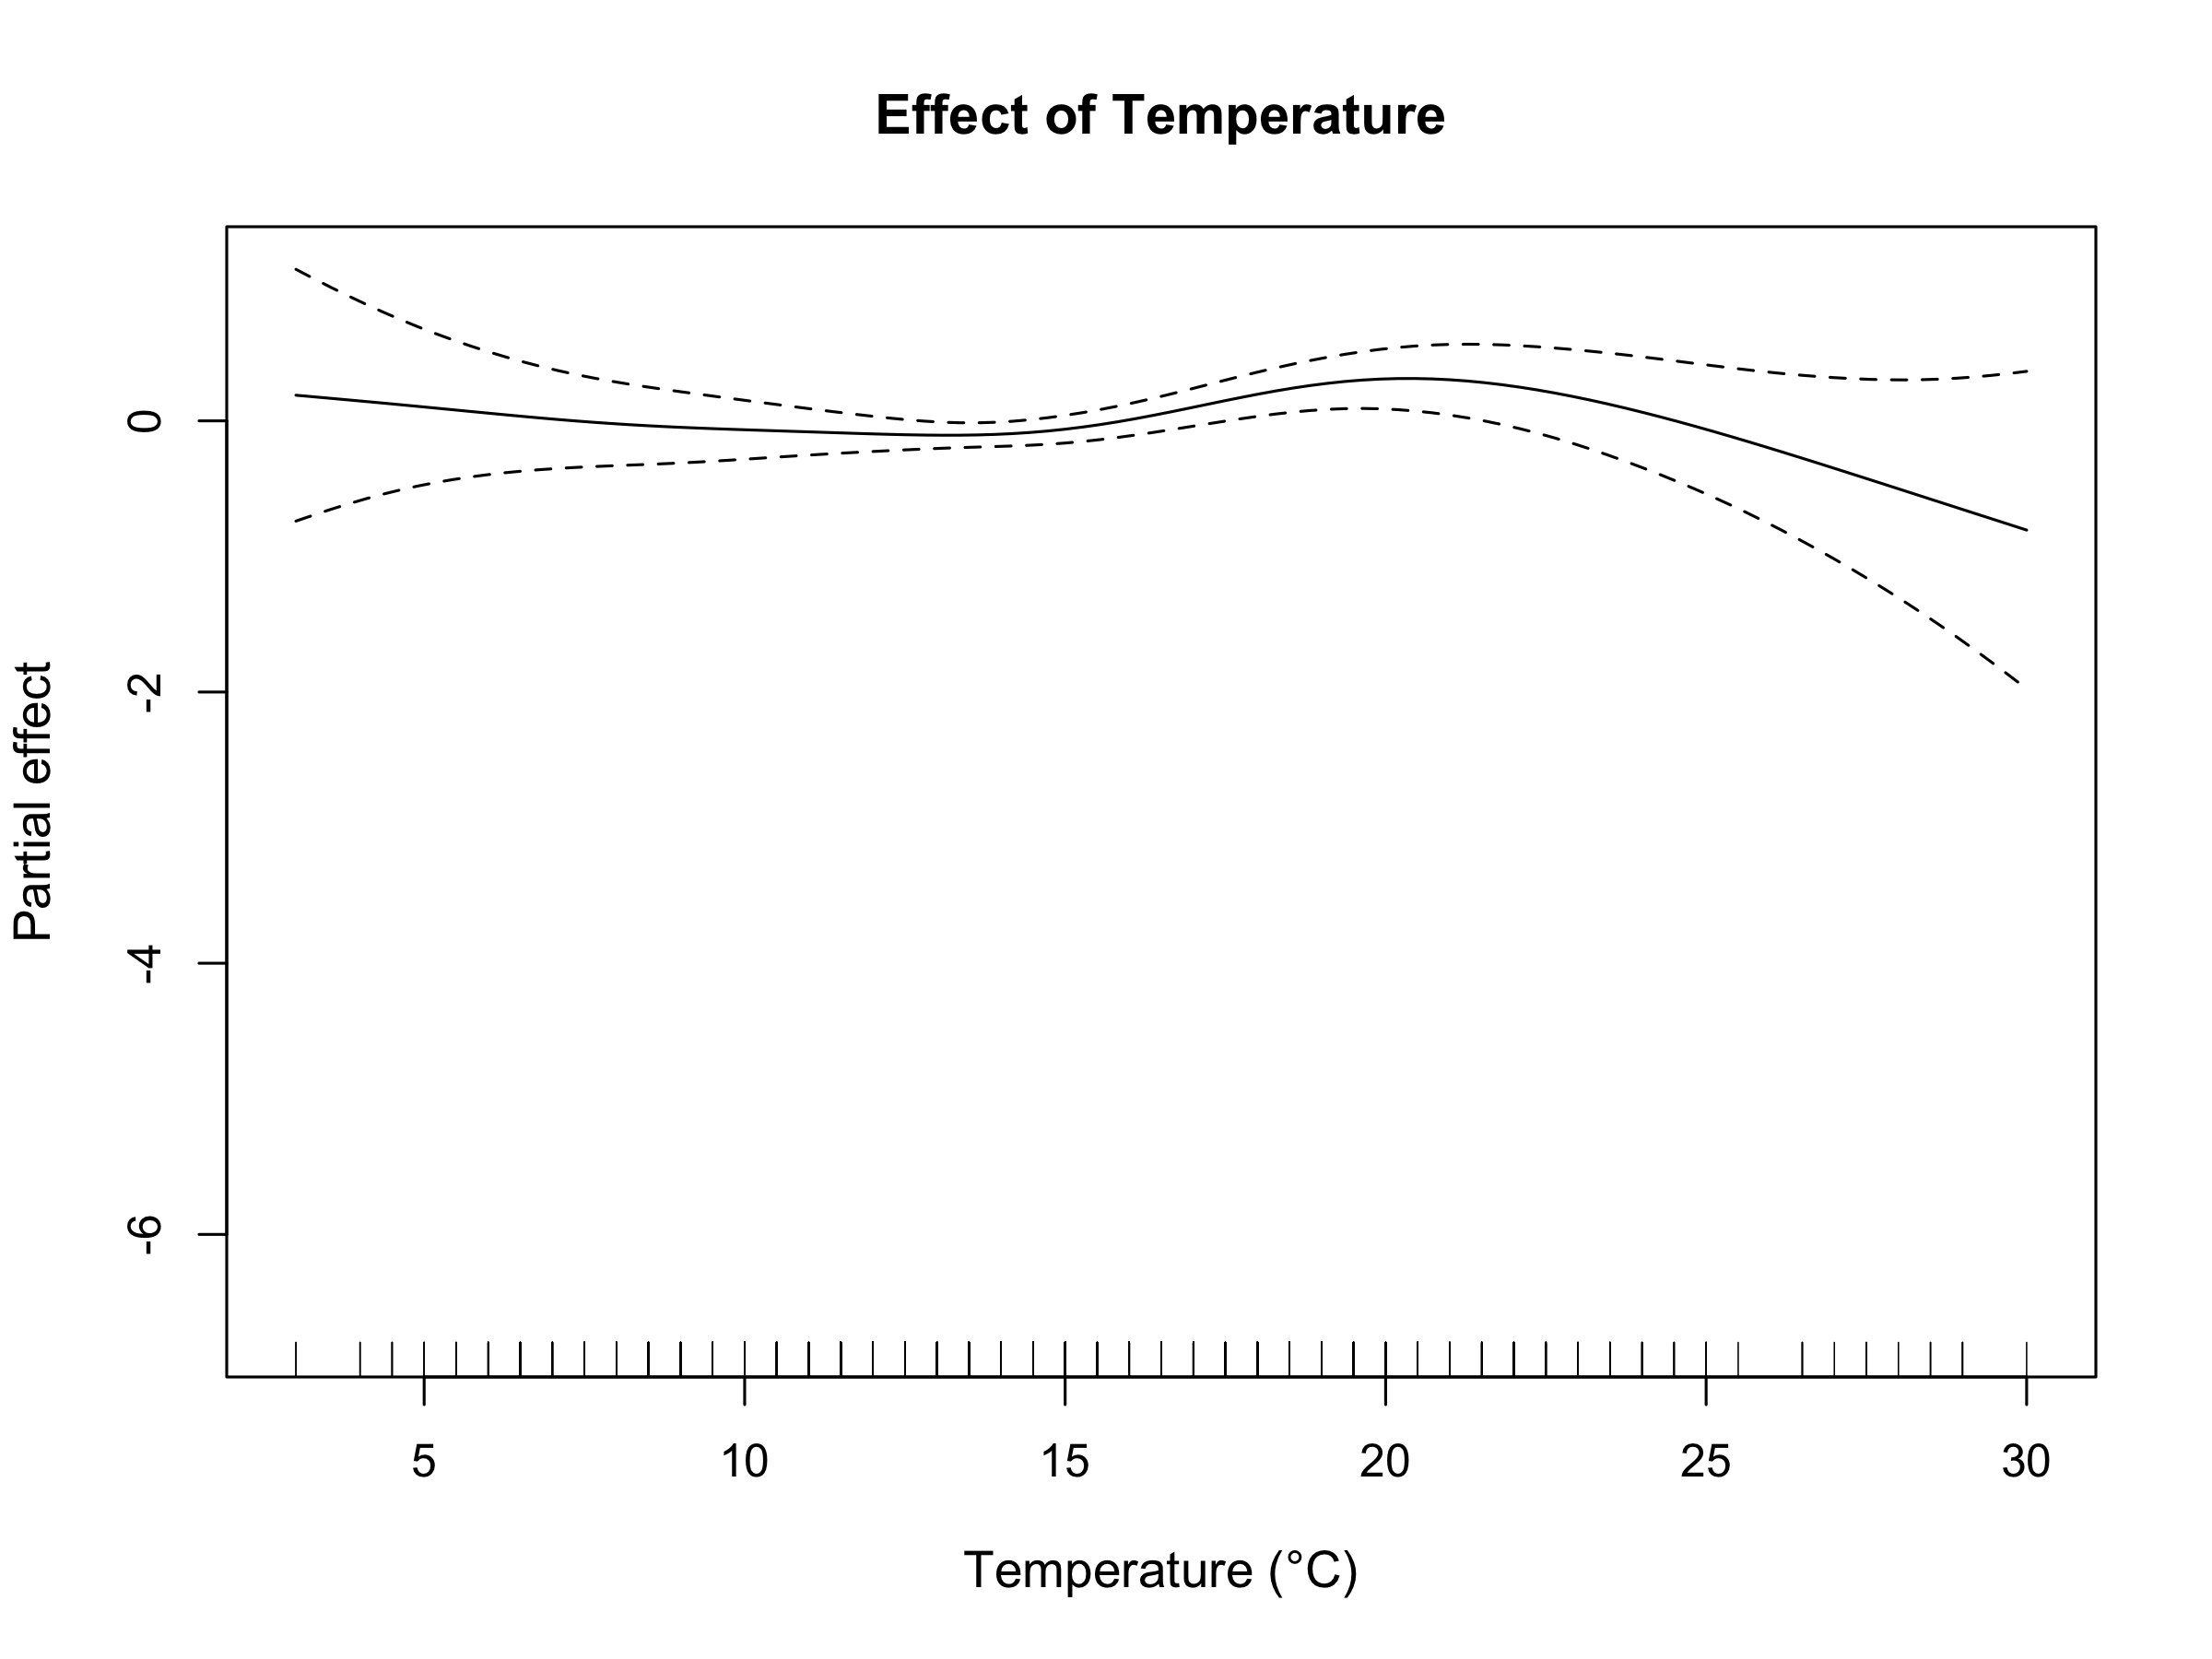
\includegraphics[width=0.8\textwidth]{supplemental/results/thesis_exports/figures/effect_temperature.png}
\caption{Partial effect of temperature on monarch abundance change, peaking at approximately 20°C. Shaded area: 95\% confidence interval.}\label{fig:effect_temperature}
\end{figure}

Butterflies in direct sun showed a strong negative effect on roost abundance (EDF = 1.53, F = 19.36, p < 0.001), with greater numbers in direct sun associated with larger decreases in total abundance (Figure~\ref{fig:effect_sun}). Time since sunrise revealed a pronounced diurnal pattern (EDF = 4.90, F = 8.90, p < 0.001), capturing cyclical changes in monarch activity throughout the day (Figure~\ref{fig:effect_diurnal}).

\begin{figure}[htbp]
\centering
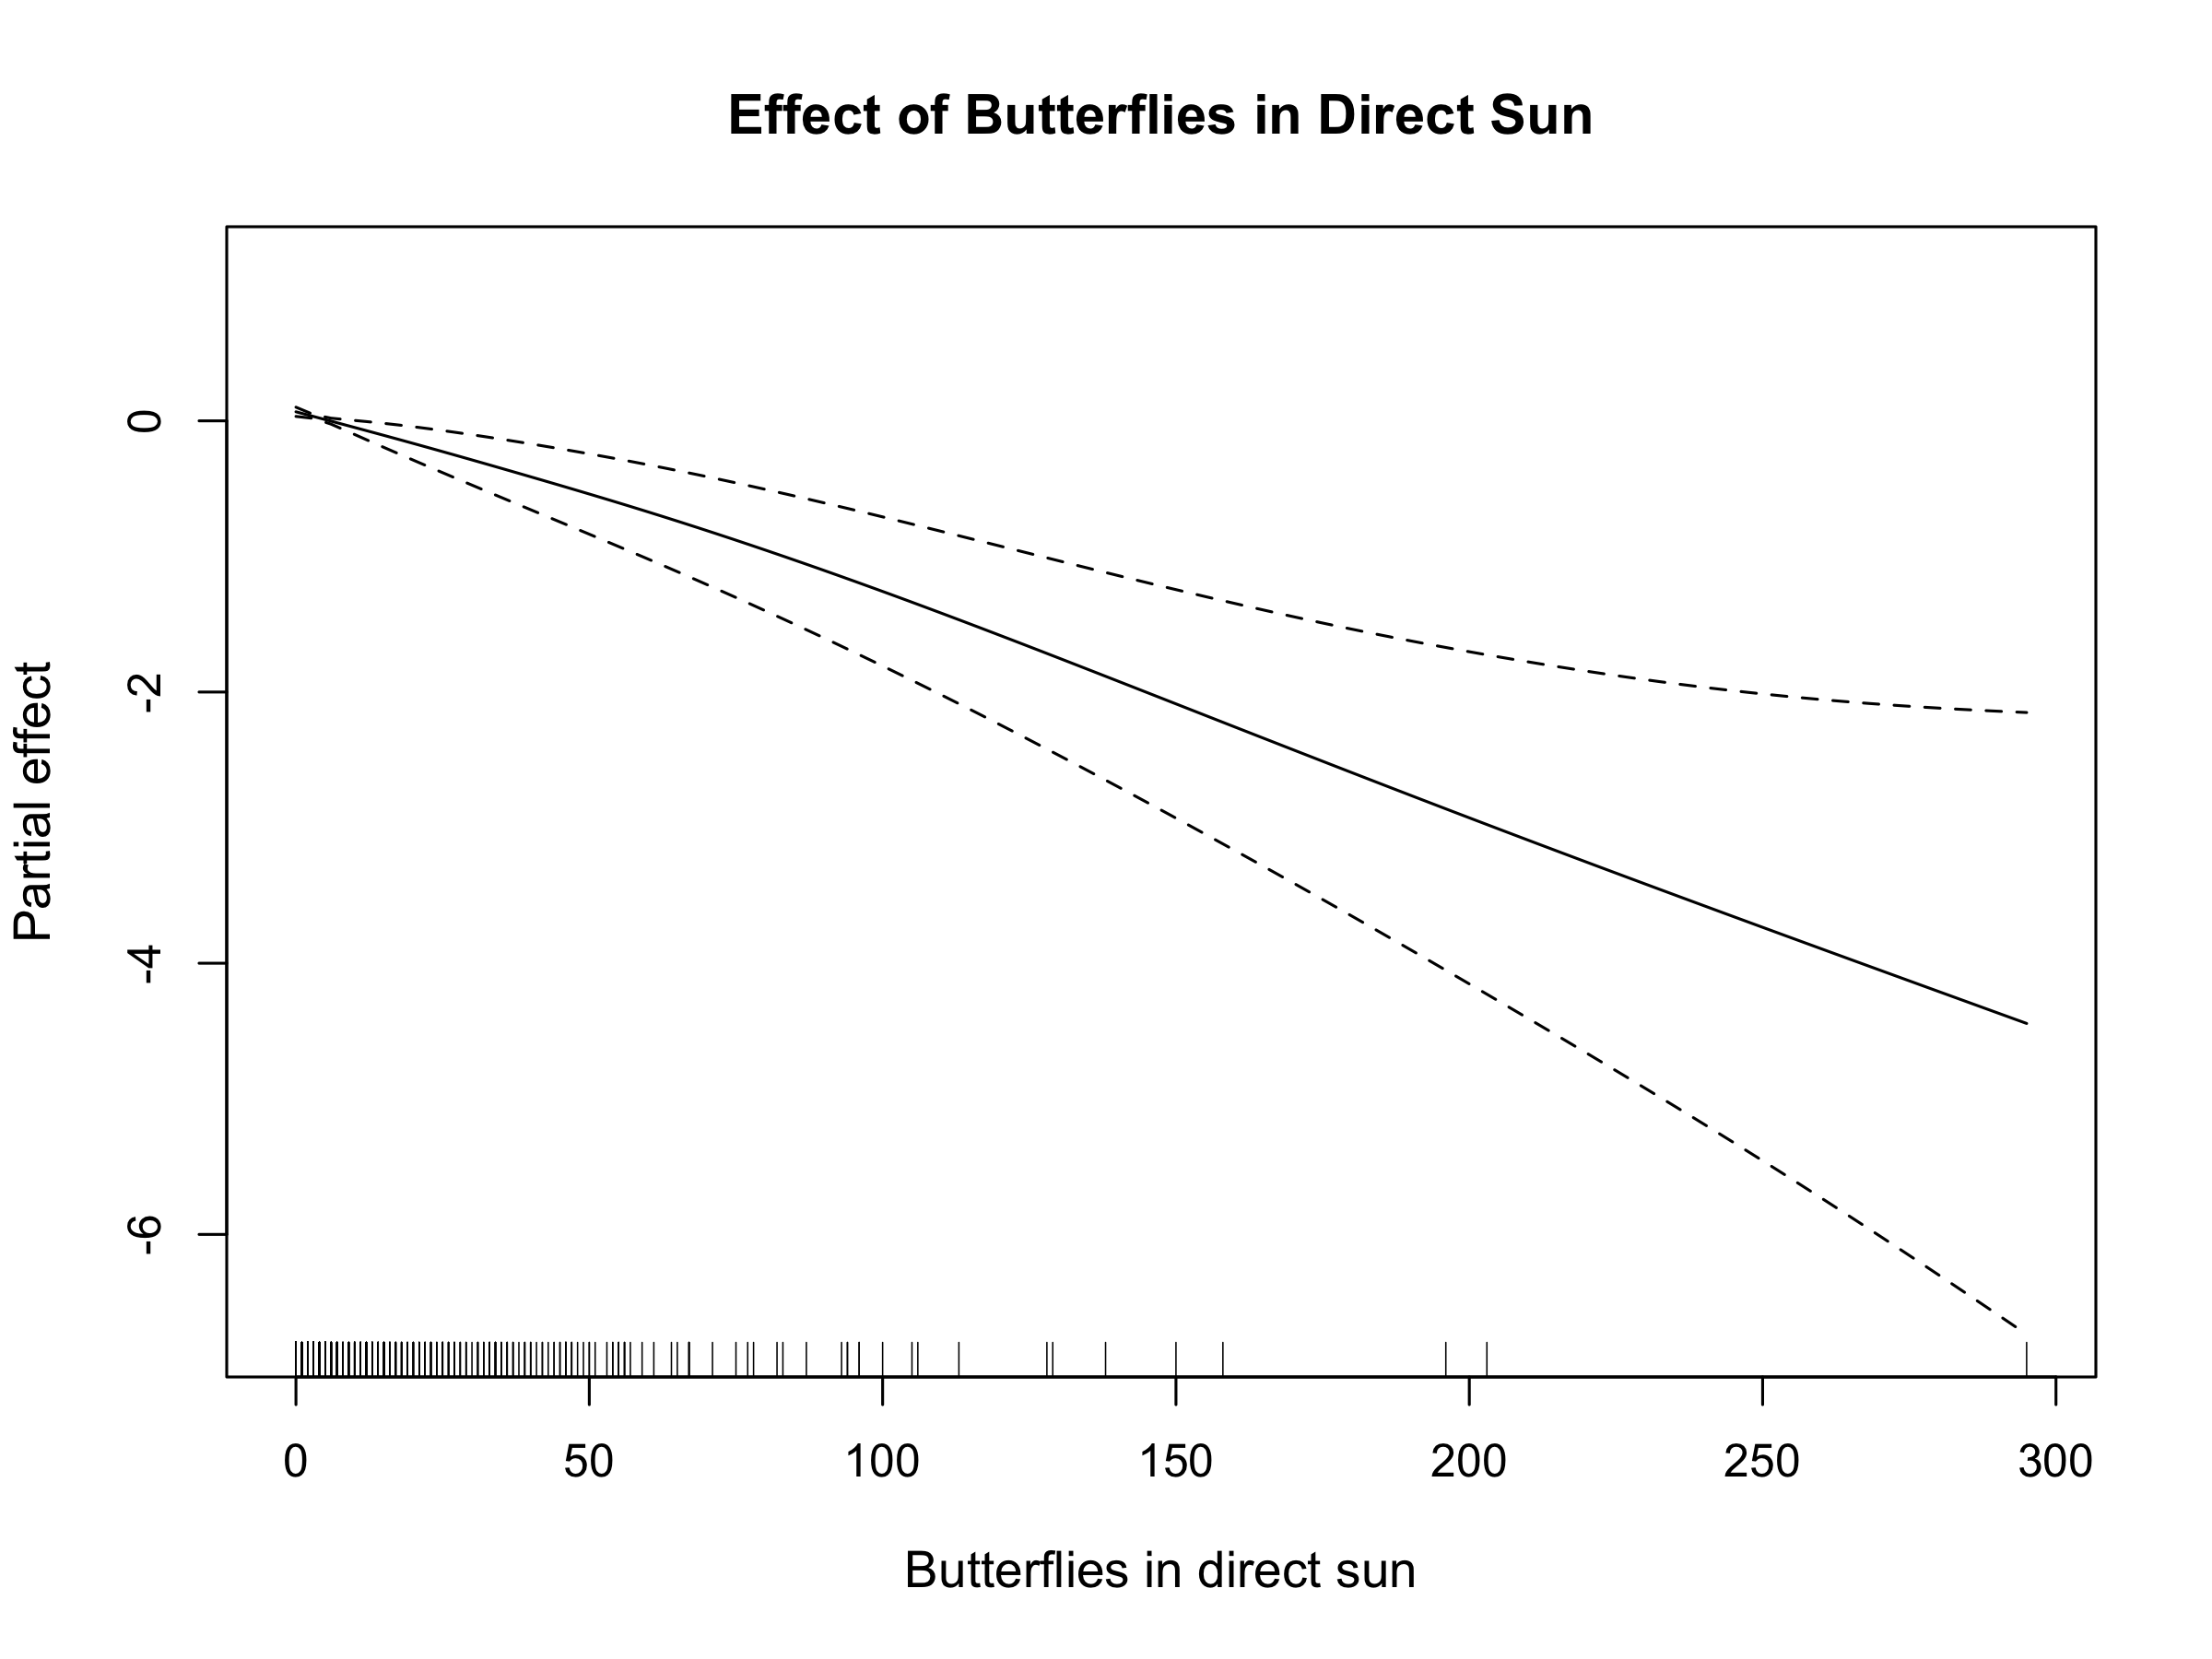
\includegraphics[width=0.8\textwidth]{supplemental/results/thesis_exports/figures/effect_butterflies_direct_sun.png}
\caption{Partial effect of butterflies in direct sun on abundance change. Greater numbers in direct sun drive departures from the roost. Shaded area: 95\% confidence interval.}\label{fig:effect_sun}
\end{figure}

\begin{figure}[htbp]
\centering
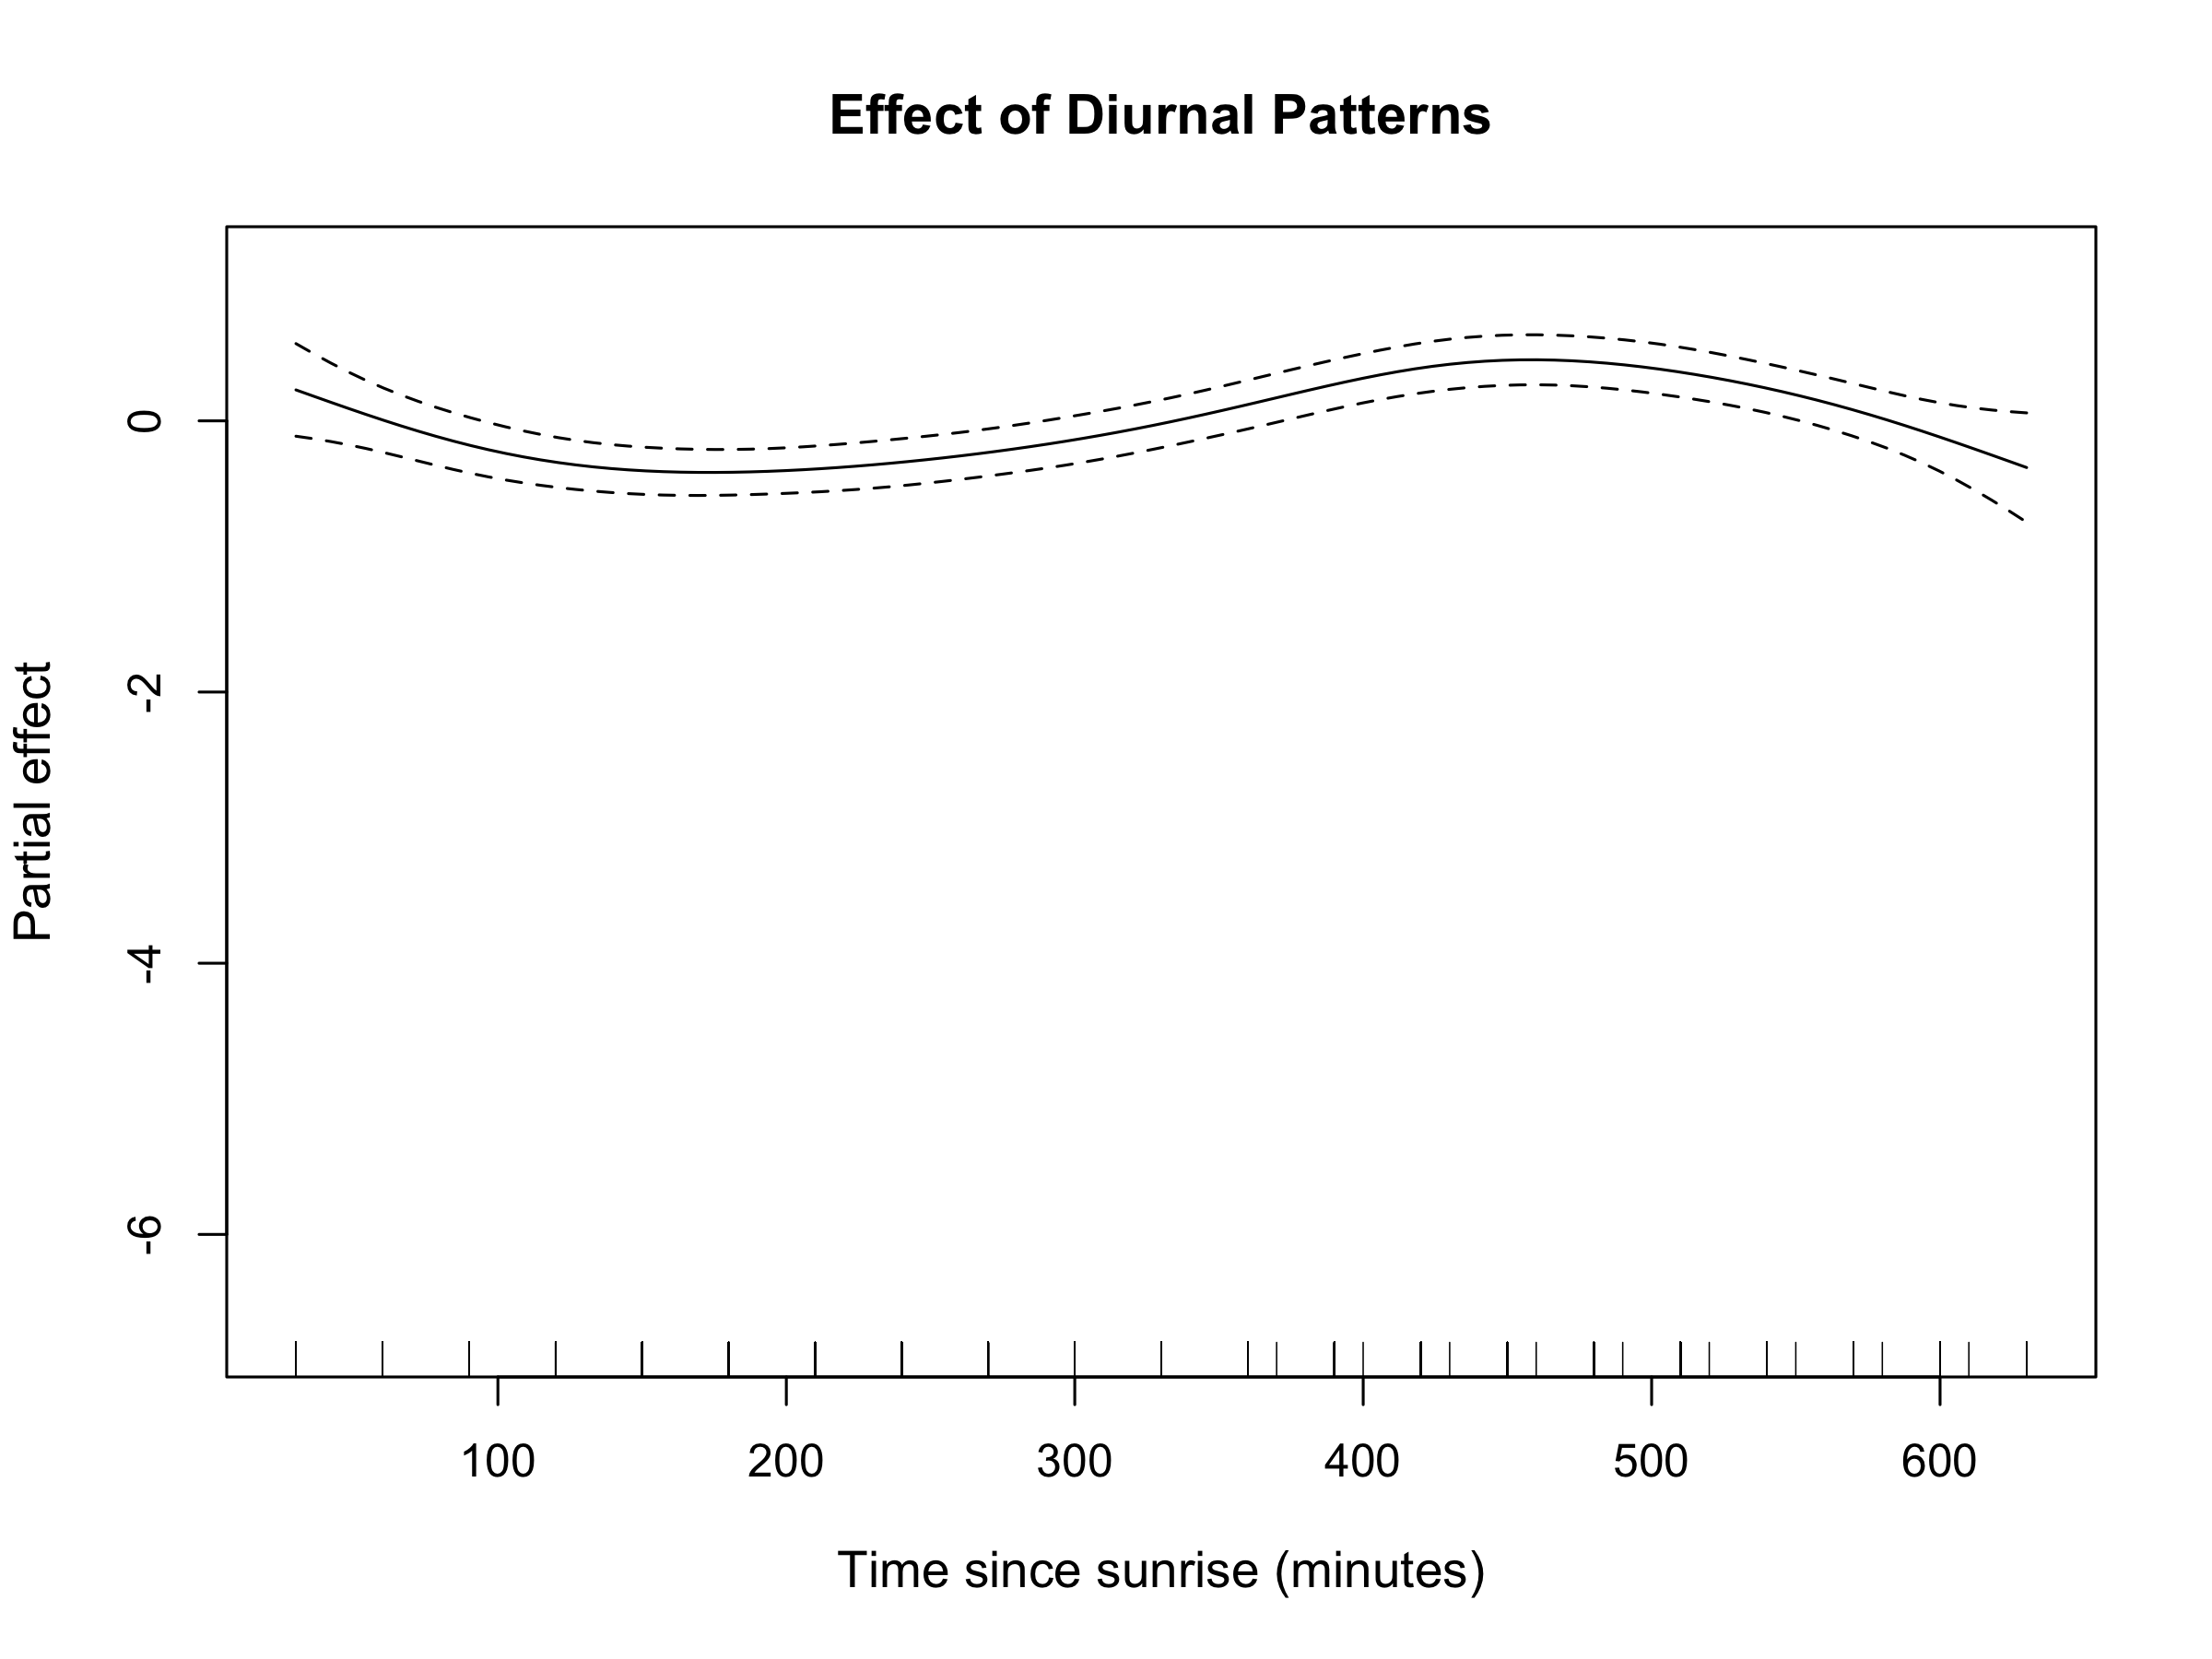
\includegraphics[width=0.8\textwidth]{supplemental/results/thesis_exports/figures/diurnal_patterns.png}
\caption{Diurnal pattern of monarch abundance changes relative to time since sunrise. Shaded area: 95\% confidence interval.}\label{fig:effect_diurnal}
\end{figure}

\subsection{Evaluation of the Disruptive Wind Hypothesis}

Our analysis provided no support for the three hierarchical wind hypotheses:

First, wind did not act as a disruptive force to overwintering monarchs. Wind variables failed to appear in any top-performing models. When maximum wind speed was forced into the best model structure (M24), model performance declined (ΔAIC = 6.2) and the wind effect was not statistically significant (p = 0.218).

Second, we found no evidence for disruption above the proposed 2~m/s threshold. With mean maximum wind speeds of 2.2~m/s (SD = 1.4~m/s)—conditions that should have revealed threshold effects if present—no disruption occurred at or above this boundary.

Third, wind's effects did not scale with intensity. The relationship remained flat across all observed wind speeds (0–12~m/s), with confidence intervals consistently encompassing zero (Figure~\ref{fig:wind_scatter}).

\begin{figure}[htbp]
\centering
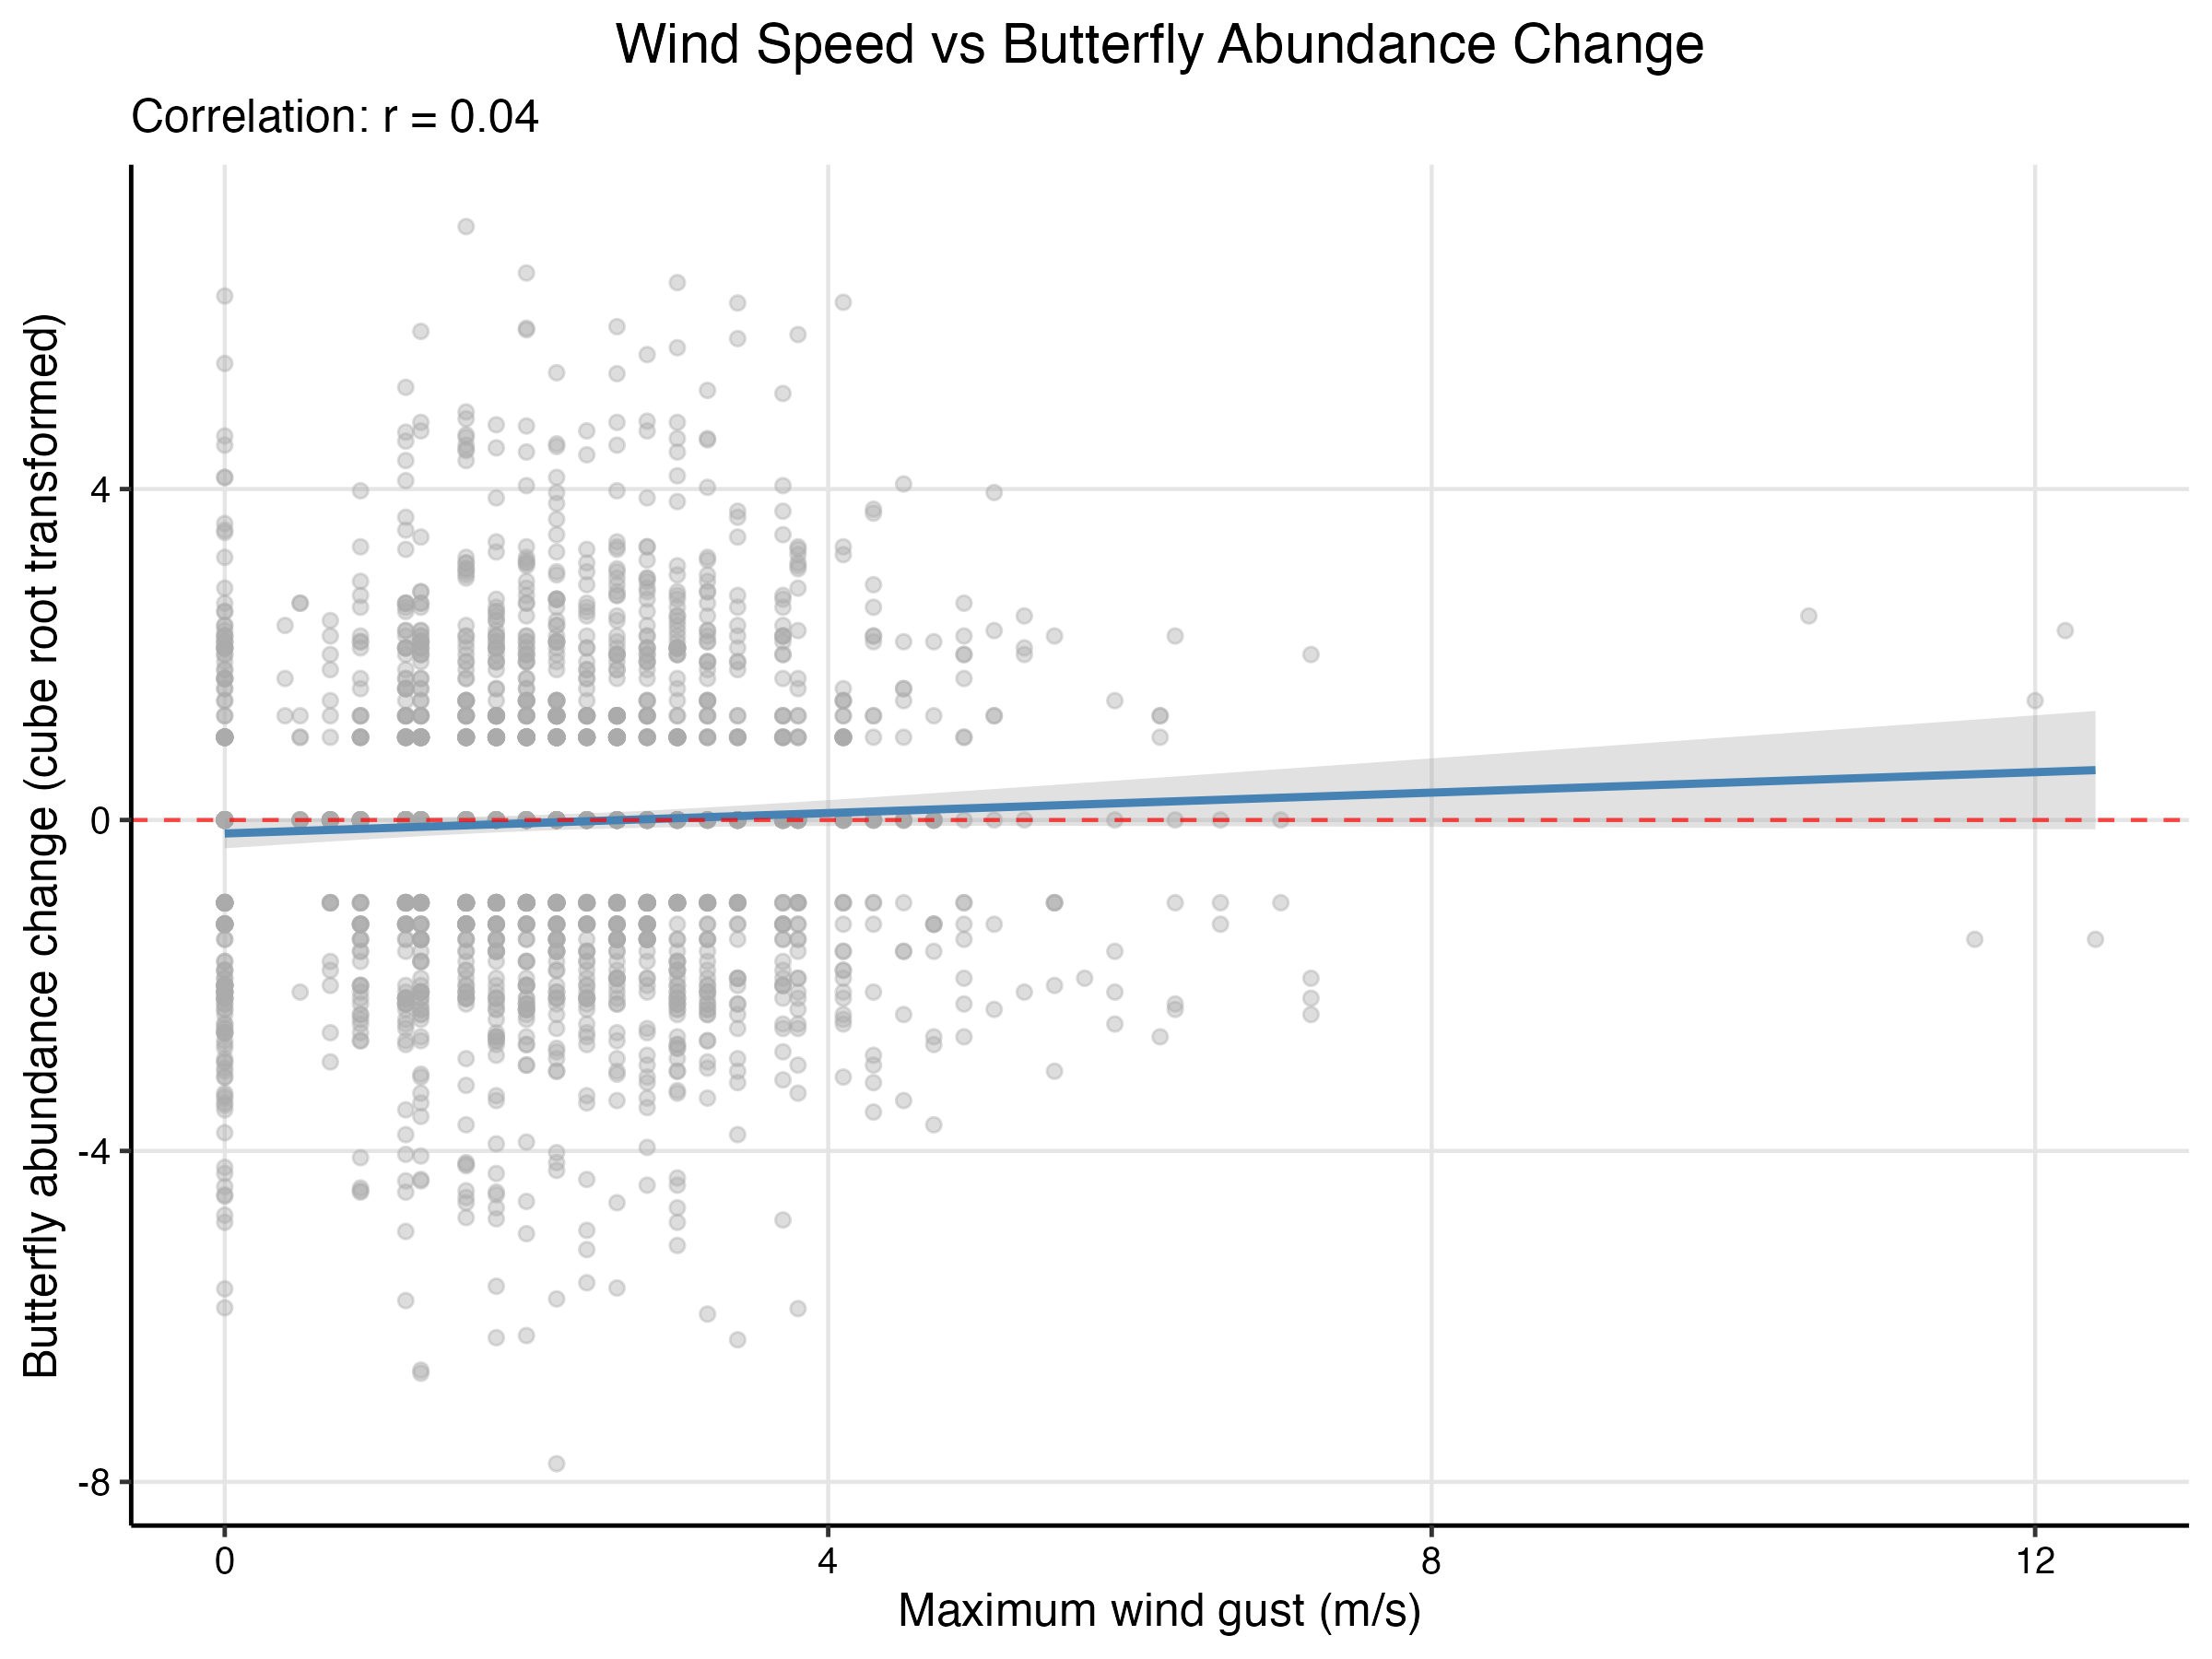
\includegraphics[width=0.8\textwidth]{supplemental/results/thesis_exports/figures/wind_hypothesis_scatter.png}
\caption{Relationship between maximum wind speed (m/s) and monarch abundance change. The red dashed line shows the proposed 2 m/s disruptive wind threshold, while the flat trend line indicates no effect of wind on butterfly departures. Points represent 30-minute observation periods.}\label{fig:wind_scatter}
\end{figure}

\subsection{Model Diagnostics}

Model residuals showed distinct linear banding patterns consistent with the discrete counting method used to estimate butterfly abundance (Figure~\ref{fig:residuals}).

\begin{figure}[htbp]
\centering
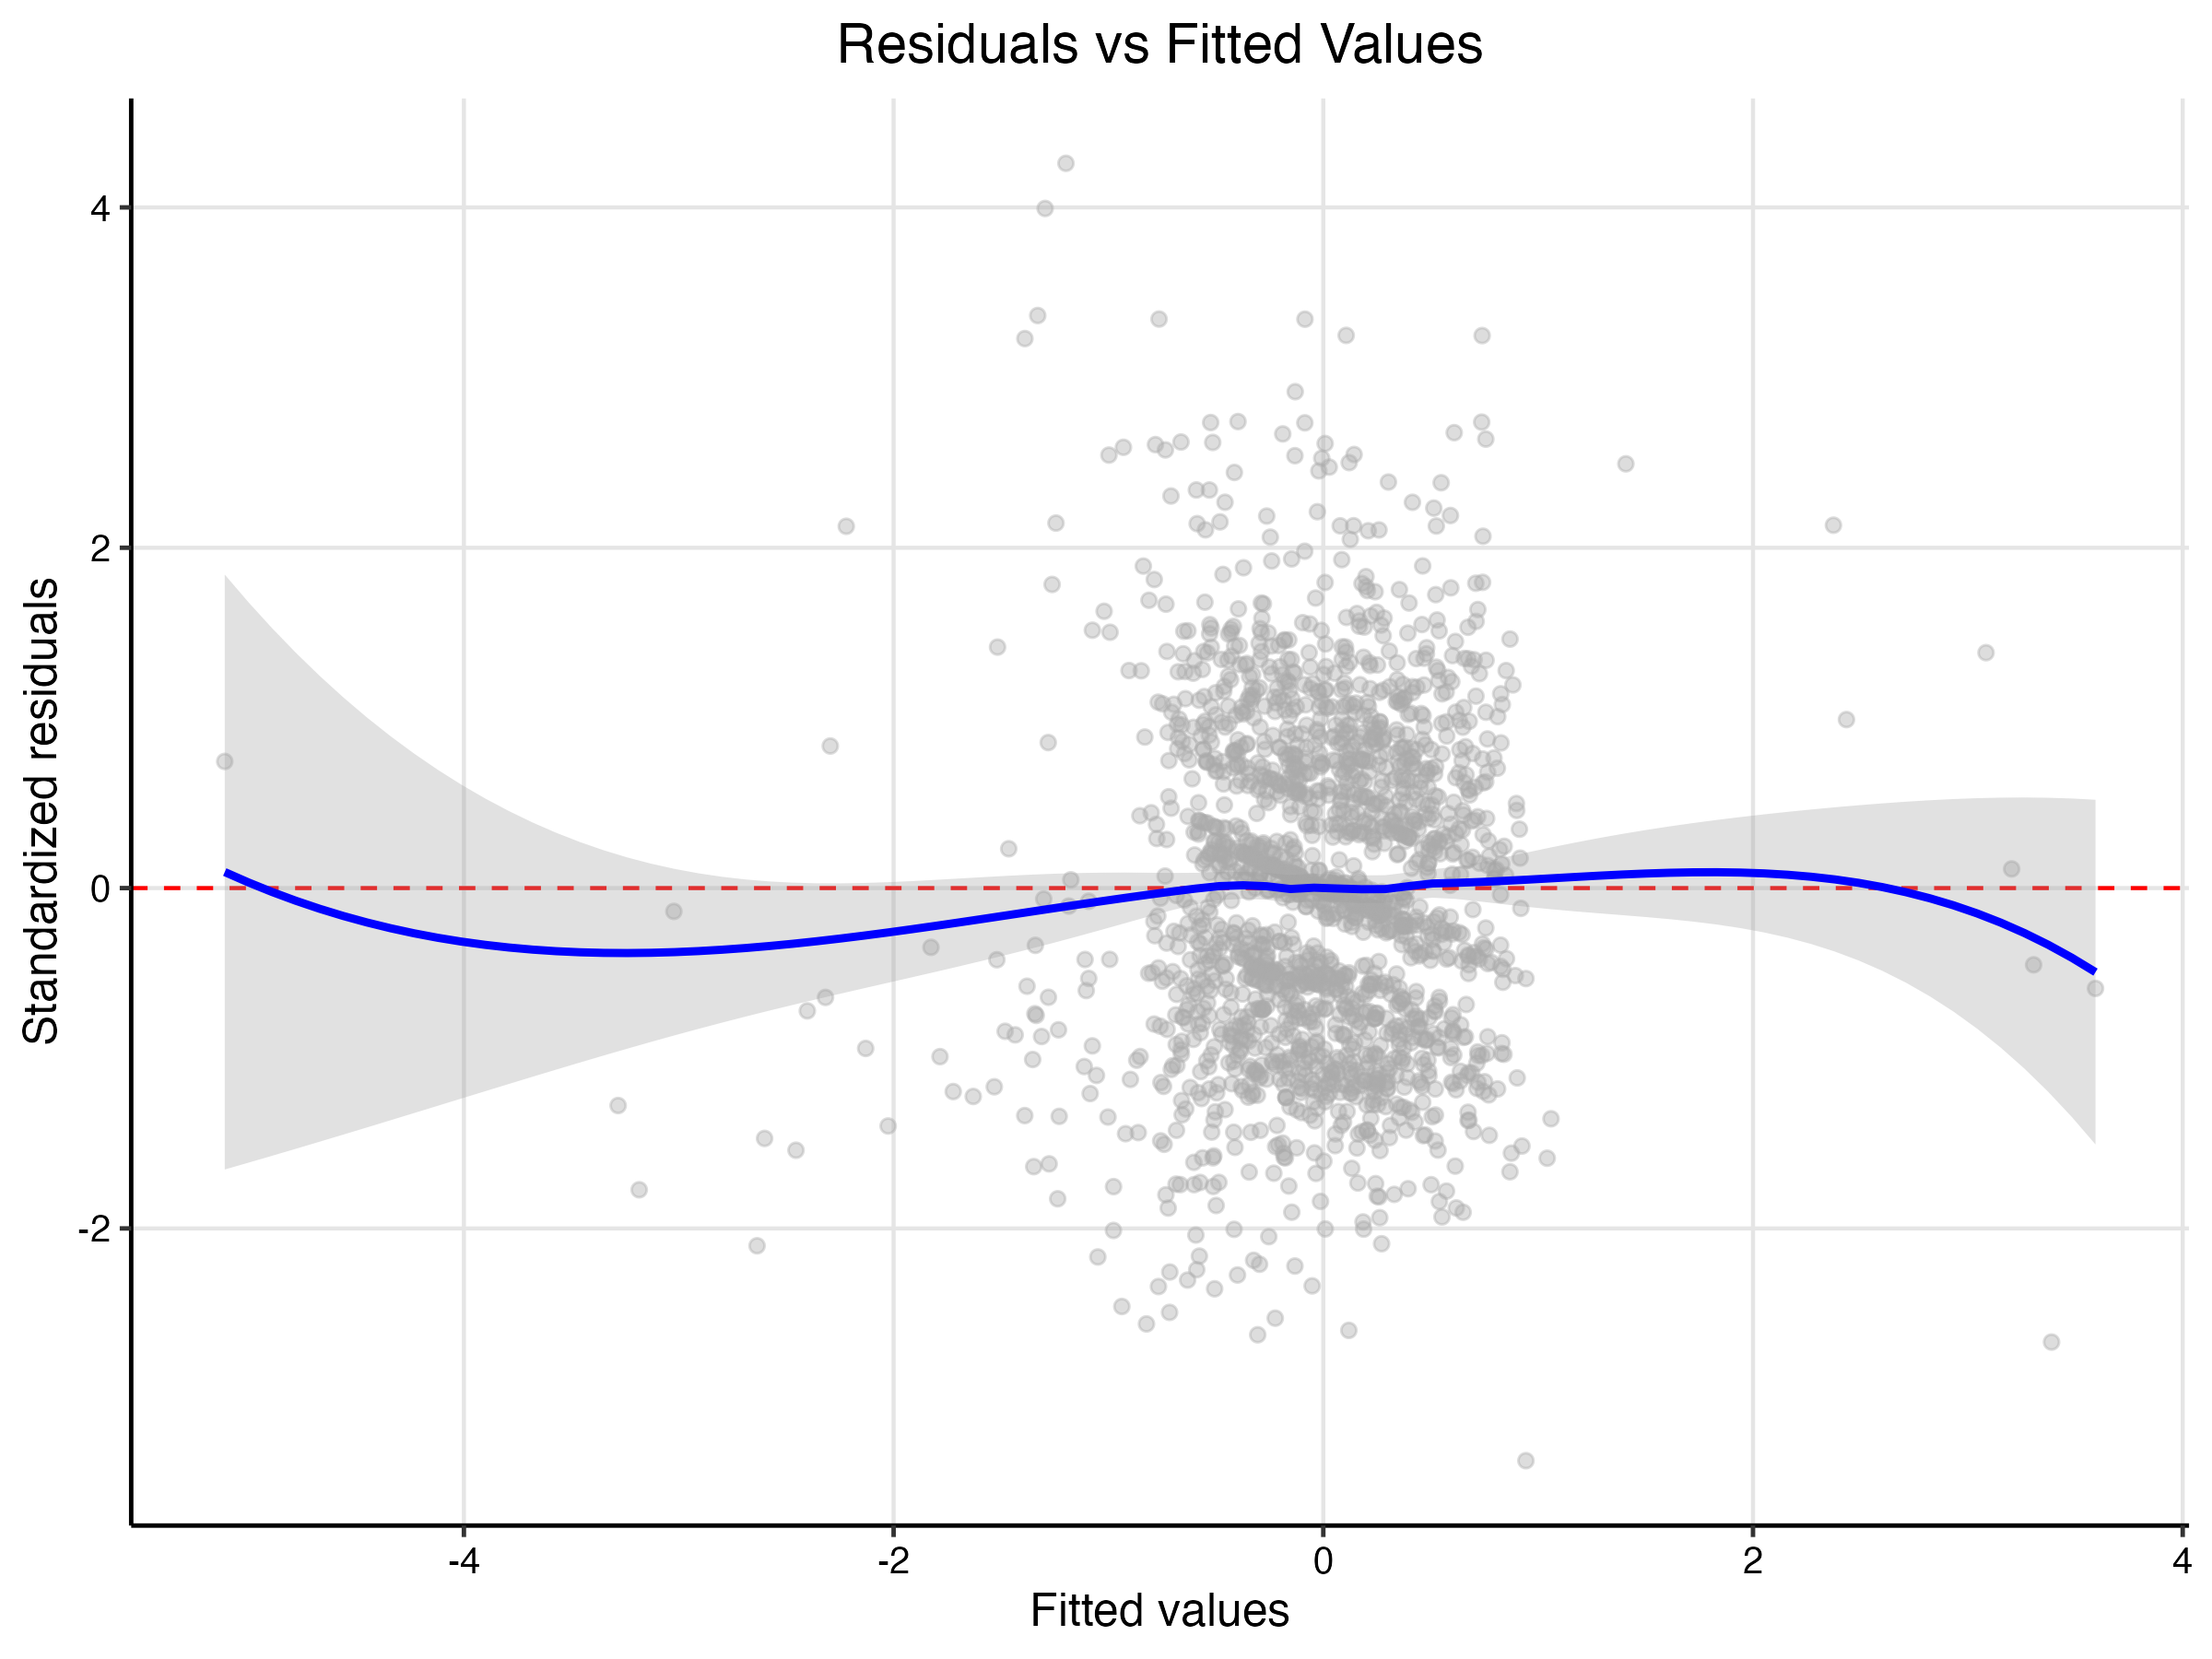
\includegraphics[width=0.8\textwidth]{supplemental/results/thesis_exports/figures/residuals_vs_fitted.png}
\caption{Residuals versus fitted values for model M23. Banding reflects the discrete counting method. Red line: smoothed relationship.}\label{fig:residuals}
\end{figure}

The Q-Q plot indicated approximately normal residual distribution with minor tail deviations (Figure~\ref{fig:qqplot}).

\begin{figure}[htbp]
\centering
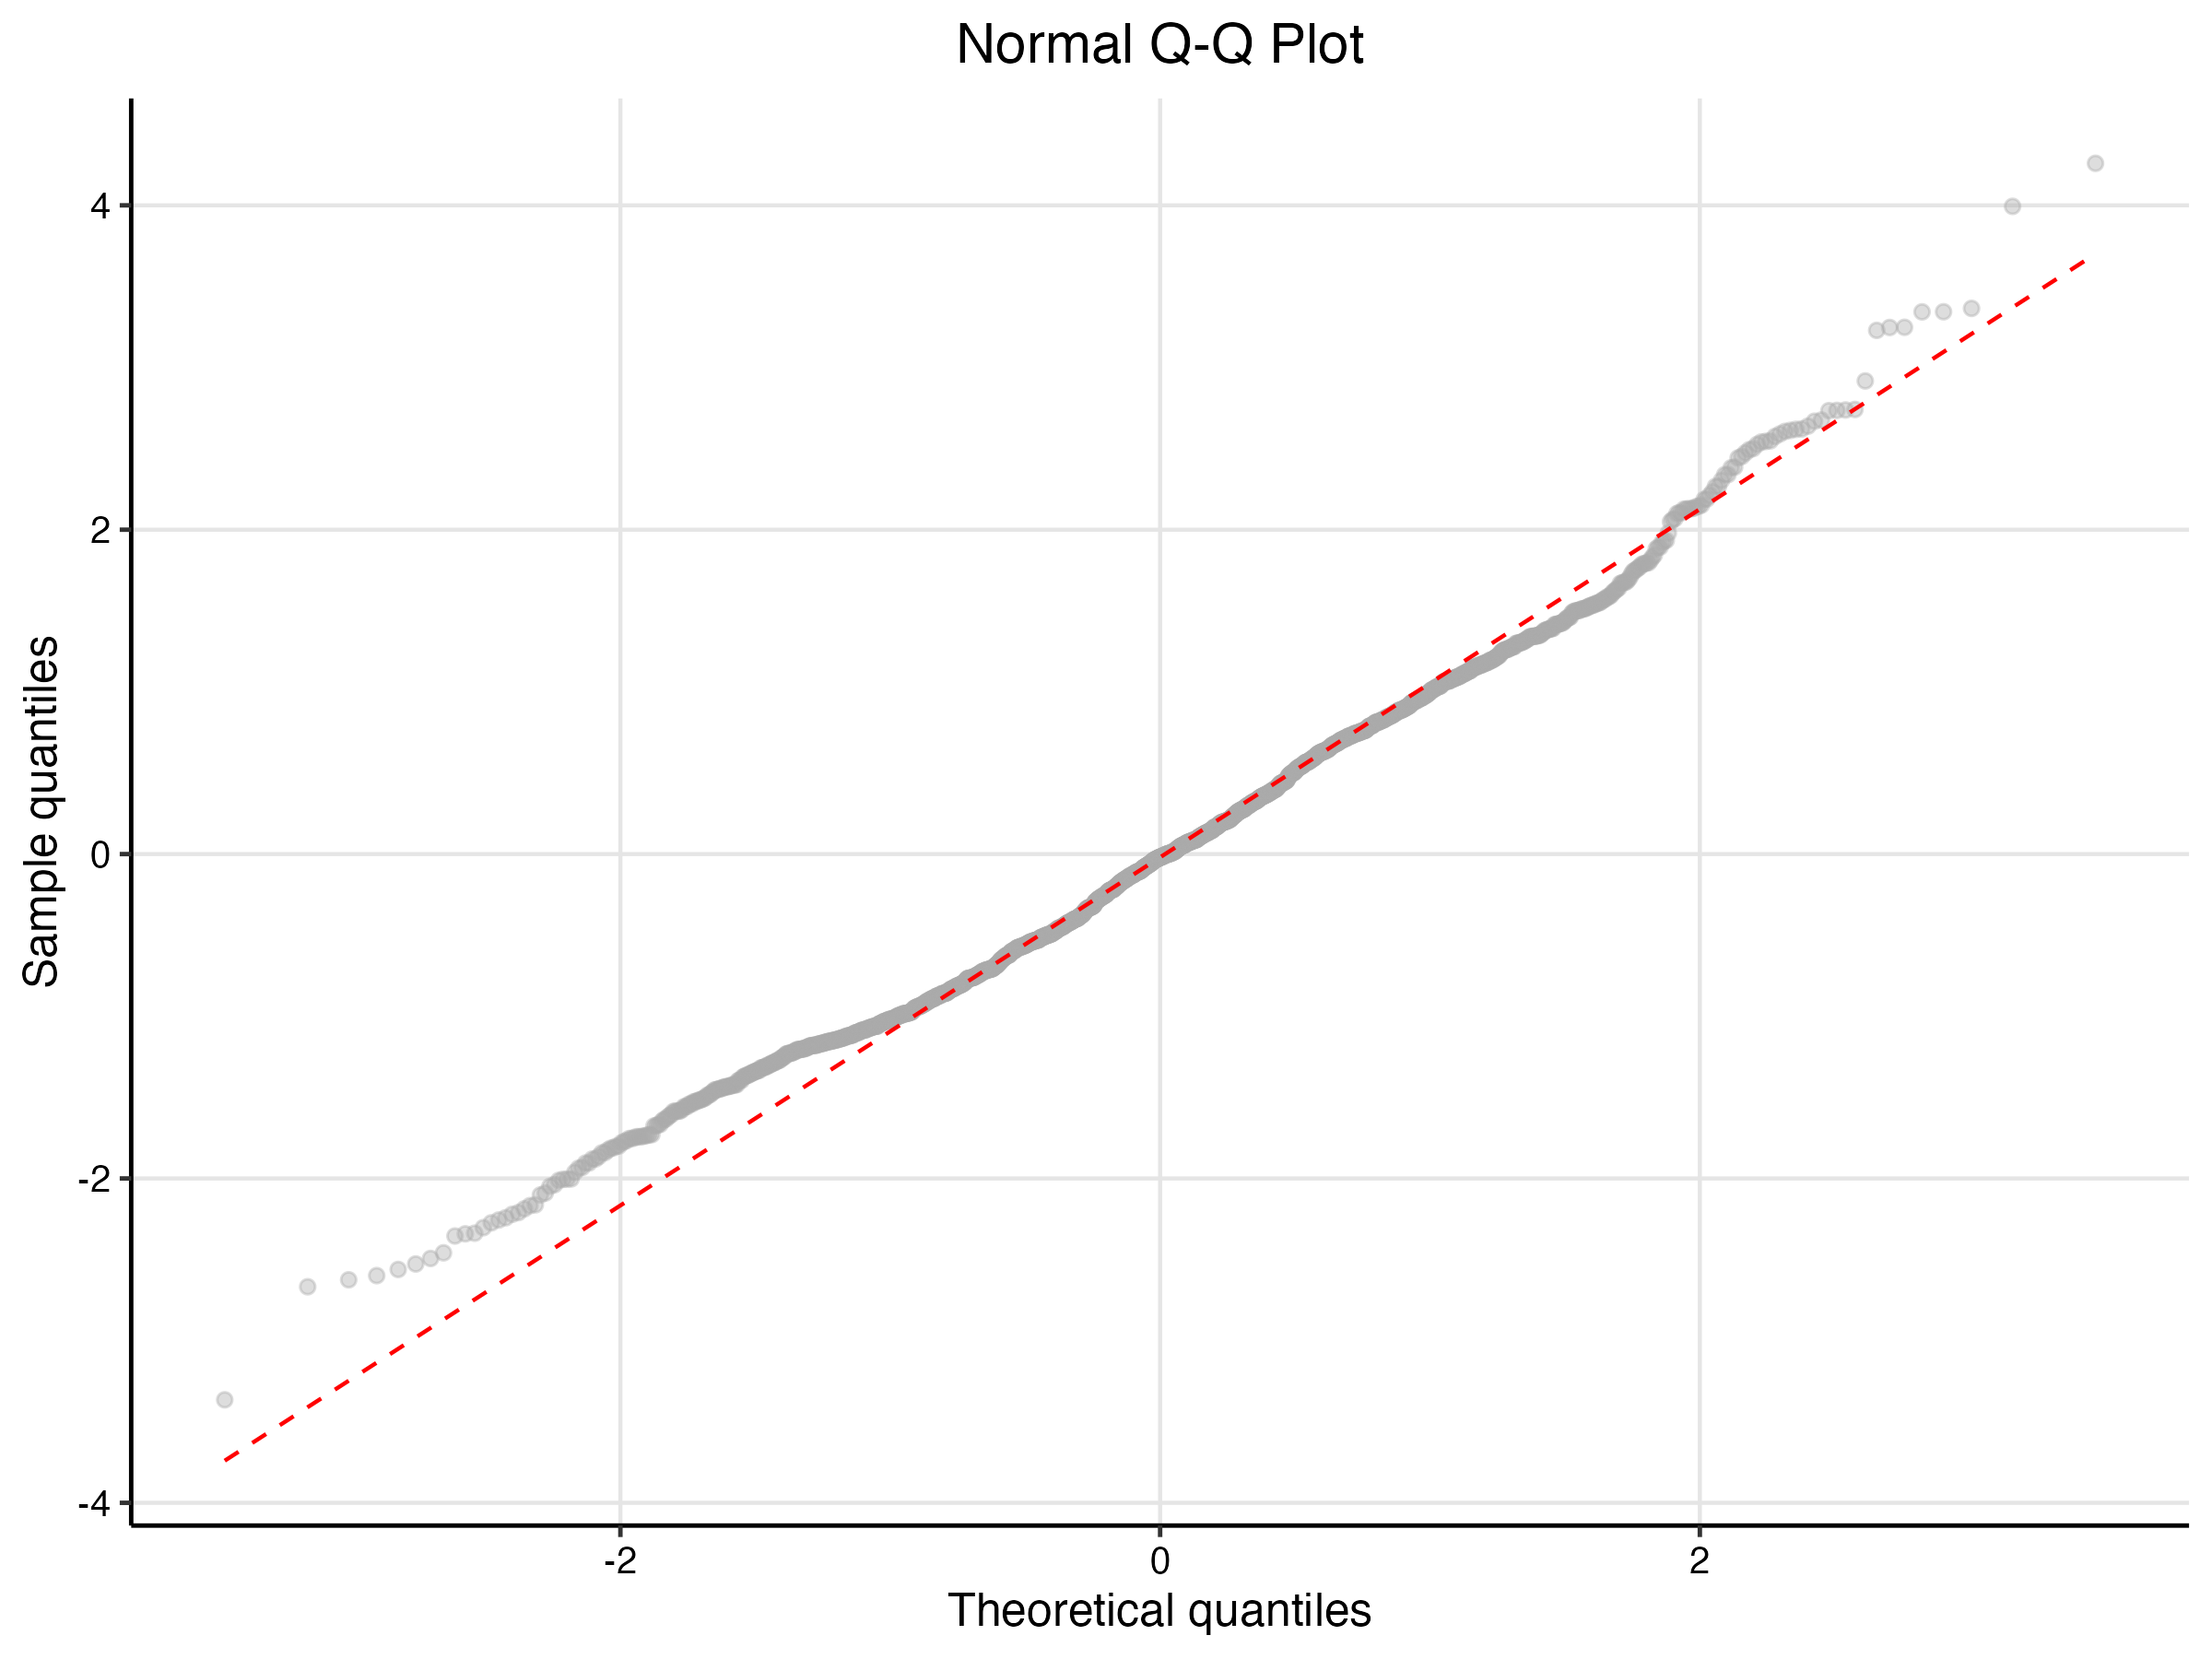
\includegraphics[width=0.8\textwidth]{supplemental/results/thesis_exports/figures/qq_plot.png}
\caption{Q-Q plot of model residuals showing reasonable normality with minor tail deviations.}\label{fig:qqplot}
\end{figure}

% To update figures, rerun the quarto doc masters-analysis/analysis/monarch_gam_analysis.qmd (separate repo) and copy the thesis-exports folder to this one.